% -----------------------------------------------------------------------------
% ########################
% # PREDLOGA ZA POROCILO #
% ########################
%
% @author Iztok Starc
% @date   3. december 2008
%
\documentclass[a4paper,12pt]{report}

% -----------------------------------------------------------------------------
% ####################################################
% # UPORABA PAKETOV - NASTAVITEV JEZIKA in KODIRANJA #
% ####################################################
\usepackage[slovene]{babel}
\usepackage[utf8]{inputenc}
\usepackage{lmodern}
\usepackage[T1]{fontenc}
\usepackage{iwona}

% -----------------------------------------------------------------------------
% ######################################
% # VNOS KLJUCNIH PARAMETROV BESEDILA  #
% ######################################

\newcommand{\naslov}     {Cake Shop}
\newcommand{\prviavtor}  {Aleš Matijevič}
\newcommand{\prviindeks} {63000214}
\newcommand{\drugiavtor} {Igor Jončevski}
\newcommand{\drugiindeks}{63070420}
\newcommand{\tretjiavtor}{Mia Erbus}
\newcommand{\tretjiindeks}{63050184}
\newcommand{\kraj}       {Ljubljana}

% -----------------------------------------------------------------------------
% ###################
% # UPORABA PAKETOV #
% ###################
\usepackage[a4paper,left=25mm,right=25mm,top=20mm,bottom=30mm,includehead]{geometry}

\usepackage{graphicx, epsfig}

\usepackage{fancyhdr}

\usepackage[
colorlinks=true, linkcolor=blue, citecolor=red,
%
pdftitle={\naslov},
pdfauthor={\prviavtor, \drugiavtor},
pdfsubject={Poročilo seminarske naloge pri predmetu Elektronsko Poslovanje},
pdfkeywords={spletna prodajalna, PHP, SSL, MySQL}, a4paper, pagebackref=true, unicode]{hyperref}

% -----------------------------------------------------------------------------
\begin{document}

% -----------------------------------------------------------------------------
% ##################
% # NASLOVNA STRAN #
% ##################
\begin{titlepage}
	\begin{center}
	{UNIVERZA V LJUBLJANI\\[10pt] 
	FAKULTETA ZA RAČUNALNIŠTVO IN INFORMATIKO}

	\vspace{65mm}

	{\Large\textbf{\naslov}}

	\vspace{10mm}

	{\large Poročilo seminarske naloge pri predmetu\\[10pt] Elektronsko poslovanje}

	\vfill
	\vspace{60mm}

\hspace{20mm}
\begin{minipage}[t]{70mm}
	{\bf Študenti}\\
	{\prviavtor} ({\prviindeks})\\ 
	{\drugiavtor} ({\drugiindeks})\\
	{\tretjiavtor} ({\tretjiindeks})
\end{minipage}
%\hfill
\begin{minipage}[t]{50mm}
	{\bf Mentor}\\
	David Jelenc
\end{minipage}
%\hspace{20mm}

	\vspace{40mm}

	{	\kraj, \today}
	\end{center}
\end{titlepage}

% -----------------------------------------------------------------------------
% ##################
% # KAZALO VSEBINE #
% ##################

\tableofcontents
% -----------------------------------------------------------------------------
% ############
% # POVZETEK #
% ############
%\begin{abstract}
%\end{abstract}

% -----------------------------------------------------------------------------
% ##################
% # UVOD DOKUMENTA #
% ##################
\chapter{Uvod}

%{\it V uvodu podajte kratko in jedrnato predstavitev teme seminarske naloge, navedite seznam uporabljene tehnologije ter naštejte uporabljene mehanizme za nadzor dostopa.}

Izdelali smo aplikacijo CakeShop, ki jo lahko uporabljajo prodajalci tort.

\section{Uporaba tehnologij}

Pri izdelavi smo uporabili tehnologije:

\begin{itemize}
  \item PHP z ogrodjem CakePHP,
  \item SQL (natančneje MySQL),
  \item Apache2,
  \item MVC (Model View Controller) pristop,
  \item REST,
  \item ORM,
  \item CRUD,
  \item Session in
  \item GitHub za izmenjavo datotek med člani skupine.
\end{itemize}

\section{Mehanizmi za nadzor dostopa}

Mehanizmi za nadzor dostopa:
\begin{itemize}
  \item SSL/TLS/HTTPS,
  \item preverjanje avtentičnosti v podatkovni bazi z uporabniškim imenom in "hashed" geslom,
  \item preverjanje avtentičnosti strežnika z digitalnim potrdilom in 
  \item preverjenje identitete adiminstratorja in prodajalca z digitalnim potrdilom
\end{itemize}

% -----------------------------------------------------------------------------
% ###################
% # JEDRO DOKUMENTA #
% ###################

% -----------------------------------------------
\chapter{Primeri uporabe}

%{\it Kratek in jedrnat opis vlog uporabnikov ter funkcionalnosti, ki so vsaki vlogi dostopne. Če ste implementirali funkcionalnosti, ki se točkujejo z dodatnimi točkami, jih posebej izpostavite.}

Ustvarili smo tri uporabnike:
\begin{enumerate}
  \item Anonimni uporabnik
  \item Stranka
  \item Prodajalec
  \item Administrator
\end{enumerate}

\section{Anonimni uporabnik}

Vsak anonimni oz. neprijavljeni obiskovalec strani lahko brska med tortami, ki so opremljene s slikami. Implementirali smo tudi funkcijo iskanja med izdelki. Anonimni uporabnik ima možnost registracije uporabniškega imena in prijave.

\section{Stranka}

Ko se anonimni uporabnik prijavi, postane prijavljen uporabnik oz. stranka. Podobno kot anonimni uporabnik, brska med izdelki. Ko se odloči za nakup izdelka, se izvede dodajanje izdelka v košarico. V košarici lahko določi, koliko primerkov tega izdelka želi, v primeru, da si premisli, lahko izdelek tudi izbriše iz košarice. Ko je stranka zadovoljna z urejanjem izdelkov, gredo izdelki na blagajno (check-out).

\section{Prodajalec}

Prodajalec ima možnost dodajanja in urejanje izdelkov, urejanja naročil in dodajnja in urejanja strank.

\section{Administrator}

Administrator ima možnost dodajanja in urejanja prodajalcev ter strank.

\section{Dodatne funkcionalnosti}

Impletirali smo tudi nekaj dodatnih funkcij, in sicer:

\begin{itemize}
  \item iskanje izdelkov,
  \item razdelitev prikaza izdelkov na posamezne strani (paginacija),
  \item predstavitev izdelkov s slikami in
  \item CSS lepotičenje.
\end{itemize}

Iskanje deluje z uporabo SQL pogoja LIKE po naslovu in opisu izdelka.

Za preglednejši pregled nad izdelki smo s pomočjo CakePHP funkcije implementirali paginacijo izdelkov. Stranke in prodajalci lahko brskajo med izdelki tako, da se s kliki pomikajo naprej in nazaj.

Predstavitev s slikami. V podatkovni bazi smo dodali tabelo slik. Vsak izdelek je lahko predstavljen brez slike (v tem primeru se mu dodeli privzeta slika), lahko pa z večimi slik, od katerih je samo ena prikazna. Vsak uporabnik lahko tudi naloži sliko s svojega računalnika.

Dodali smo tudi CSS datoteko za vsak pogled (pogled stranke, prodajalca in administratorja.

% -----------------------------------------------
\chapter{Uporabniške pristopne točke}

%{\it Opis uporabniških pristopnih točk. Tukaj lahko dokumentirate uporabniški vmesnik za ključne primere uporabe, tako da zajamete zaslonske slike vaše aplikacije in jih opremite s komentarji.}

\section{Prijava}

Uporabnik se prijavi v sistem.

\begin{figure}[htb]
	\centering
	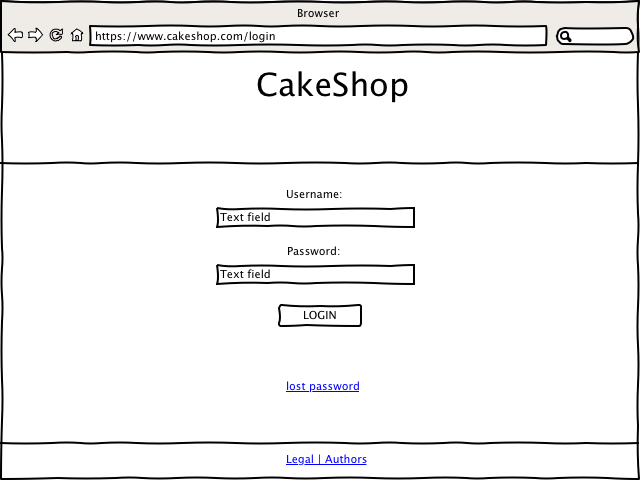
\includegraphics[width=13cm]{Wireframes/cakeshop/pngs/010200-LoginAnonymous.png}
	\caption{Prijava}
\label{fig:1}
\end{figure}

\newpage

\section{Prikaz izdelkov}

Prikaz izdelkov s slikami in paginacijo.

\begin{figure}[htb]
	\centering
	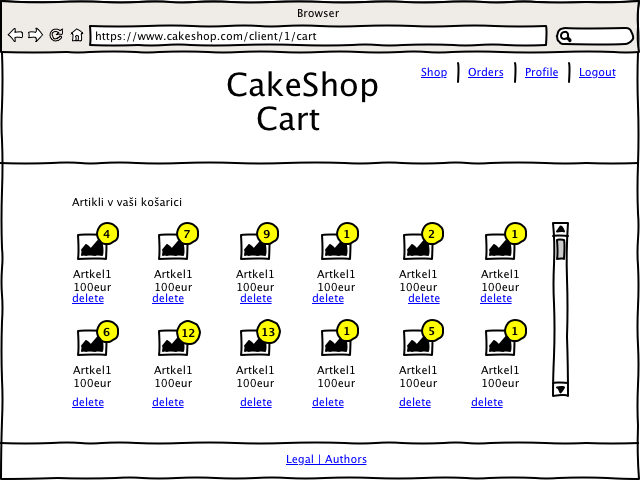
\includegraphics[width=13cm]{Wireframes/cakeshop/pngs/020200-CartViewClient.png}
	\caption{Košarica}
\label{fig:1}
\end{figure}

\section{Dodajanje v košarico}

Dodajanje v košarico

\section{Naročila}

\begin{figure}[htb]
	\centering
	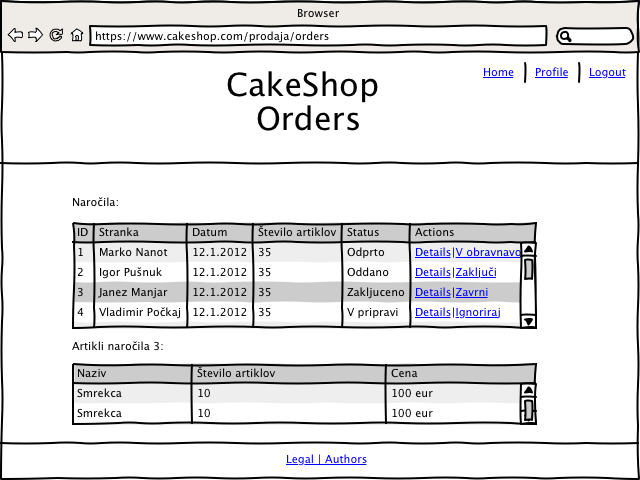
\includegraphics[width=13cm]{Wireframes/cakeshop/pngs/030300-OrdersSalesman.png}
	\caption{Košarica}
\label{fig:1}
\end{figure}

% -----------------------------------------------
\chapter{Podatkovni model}

%{\it Slika logičnega podatkovnega modela (denimo iz programa MySQL Workbench) ter kratek opis tabel in obrazložitev netrivialnih atributov.}

% -----------------------------------------------
\chapter{Varnost sistema}

{\it Opis mehanizmov nadzora dostopa in ostalih varnostnih mehanizmov implementacije (SSL/TLS, preverjanje vnosov odjemalca, CAPTCHA, uporaba regularnih izrazov, \dots).}

% -----------------------------------------------
\chapter{Izjava o avtorstvu seminarske naloge}

Spodaj podpisani \textit{\prviavtor}, vpisna številka \textit{\prviindeks}, sem (so)avtor seminarske naloge z naslovom \textit{\naslov}. S svojim podpisom zagotavljam, da sem izdelal ali bil soudeležen pri izdelavi naslednjih sklopov seminarske naloge:
\begin{itemize}
    \item Vzorčni sklop 1
	 \item Vzorčni sklop 2
\end{itemize}

Podpis: {\prviavtor}, l.r.

\newpage

Spodaj podpisana \textit{\drugiavtor}, vpisna številka \textit{\drugiindeks}, sem (so)avtor seminarske naloge z naslovom \textit{\naslov}. S svojim podpisom zagotavljam, da sem izdelal ali bil soudeležen pri izdelavi naslednjih sklopov seminarske naloge:
\begin{itemize}
    \item Vzorčni sklop 1
	 \item Vzorčni sklop 2
\end{itemize}

Podpis: {\drugiavtor}, l.r.

\newpage

Spodaj podpisana \textit{\tretjiavtor}, vpisna številka \textit{\tretjiindeks}, sem (so)avtor seminarske naloge z naslovom \textit{\naslov}. S svojim podpisom zagotavljam, da sem izdelal ali bil soudeležen pri izdelavi naslednjih sklopov seminarske naloge:
\begin{itemize}
    \item Vzorčni sklop 1
	 \item Vzorčni sklop 2
\end{itemize}

Podpis: {\tretjiavtor}, l.r.

% -----------------------------------------------
\chapter{Dodatno vzorčno poglavje}

Besedilo poglavja.

\section{Dodatni vzorčni odsek ena}

Besedilo odseka.

\section{Dodatni vzorčni odsek dva}

Besedilo odseka.

\section{Dodatni vzorčni odsek tri}

Besedilo odseka.

\begin{table}[htb]
 \centering
 \begin{tabular}{c || c}
  \textbf{N} & Vsebina\\ \hline\hline
  1 & Vrstica 1\\        \hline
  2 & Vrstica 2\\        \hline
  ... & ... \\
\end{tabular}
\caption{Tabela vrednosti vzorcev}
\label{tab:1}
\end{table}

Besedilo odseka.

\begin{figure}[htb]
	\centering
	
\includegraphics[width=13cm]{img/vzorec.jpg}
	\caption{Slika določenega vzorca}
\label{fig:1}
\end{figure}

Besedilo odseka.

% -----------------------------------------------------------------------------
% #######################
% # ZAKLJUCEK DOKUMENTA #
% #######################
\chapter{Zaključek}

Zaključek.

% -----------------------------------------------------------------------------
% ##############
% # LITERATURA #
% ##############
\begin{thebibliography}{99}
\addtocounter{chapter}{1}
\addcontentsline{toc}{chapter}{\protect\numberline{\thechapter}Literatura}
\addtocontents{toc}{\protect\vspace{15pt}}

\bibitem{bib:ref} Yank K. \emph{Build Your Own Database-Driven Website Using PHP \& MySQL}. SitePoint, 2003. ISBN-10: 0-957-92181-0.

\bibitem{bib:ref1} Michele D.; Jon P. \emph{Learning PHP and MySQL}. O'Rielly, 2006. ISBN-10: 0-596-10110-4.

\bibitem{bib:ref2} Tim C.; Joyce P.; Clark M. \emph{PHP5 and MySQL Bible}. Wiley Publishing, Inc., 2004. ISBN-10: 0-7645-5746-7

\bibitem{bib:LinuxCommandReference} Red Hat Software inc. \emph{Linux Complete Command Reference}. Sams Publishing, 1997. ISBN-10: 0-672-31104-6.

\bibitem{bib:IPsecHowTo1} Ralf Spennberg. \emph{IPsec HOWTO} (online). 2003. (citirano \today). Dostopno na naslovu:
\url{http://www.ipsec-howto.org/t1.html}

\end{thebibliography}

% -----------------------------------------------------------------------------
% ###########
% # DODATEK #
% ###########

 \appendix

\chapter{Naslov dodatka}
{\it Po potrebi.}

\end{document}
